\documentclass[conference]{IEEEtran}

\usepackage[dvips]{graphicx}
\usepackage{amsmath,amssymb}
\usepackage{algorithm}
\usepackage{algorithmic}
\usepackage{flushend}

\begin{document}
\title{IMSI-based Routing in IPX and Identity Privacy in 5G}
\date{}%date stay empty

\author{
\IEEEauthorblockN{Mohsin Khan, Valtteri Niemi}
\IEEEauthorblockA{University of Helsinki \\ Helsinki, Finland \\ {mohsin.khan, valtteri.niemi}@helsinki.fi\\}
\and
\IEEEauthorblockN{Philip Ginzboorg}
\IEEEauthorblockA{Huawei Technologies \\ Helsini, Finland \\ philip.ginzboorg@huawei.com\\}}
\maketitle

\begin{abstract}
In 5G, identity privacy of a user is proposed to be protected by concealing the identifier of the user. In order to route the concealed identifier to the appropriate destination, certain information of about the IMSI - country code and network code need to be revealed. However, only recently, it is raised that when the destination is a virtual mobile network operator or a unified data management entity, the routing in IPX needs more information about the IMSI to be revealed. In this new context, we re-examine published alternative solutions of identity privacy. We find the previously promising solutions e.g., solution based on public key of home network become less promising. We find the solution based on identity based encryption becomes more promising than it was before.
\end{abstract}

\section{Introduction} \label{intro}
One major problem in the realm of identity privacy in mobile networks is to privatize the international mobile subscriber identity (IMSI). Serious effort has been put to solve this problem in the 3GPP community. Most of the solutions are based on some cryptographic techniques. Comparative analysis between the solutions have been published. There have been pros and cons in every solution. 
3GPP community is now at the verge of finalizing the specification for the first phase of 5G network. Idneity privacy is a major requirement in 5G. A solution based on public key cryptography is most likely going to be adopted privatize IMSI. Very recently a issue of routing the IMSIs in IPX has been raised. This routing issue weakens the effectiveness of this solution. Another issue around lawful interception (LI) has been noticed only recently.

In this paper we will do the comparative analysis in the light of these two new concerns. We will see that the balance of pros and cons between different solutions change significantly. The root-key based solution which appeared to be quite straightforward and effective solution becomes less effective and requires more implementation effort. On the other hand a solution based on identity based encryption which had its own cons, now nicely solve both of the concerns of IPX routing and LI. In this light we will argue that solution based on identity based encryption is the most effective and fairly straightforward solution to privatize IMSI.

In order to present a smooth discussion, first we need to explain some background. We will present an abstract view of a mobile network - we will use LTE. We will discuss how IMSI is used, how privacy of IMSI is vulnerable. We will also discuss the published solutions to some extent. Then we will explain the new concerns around IPX routing and LI. Then we will explain how the solution based on identity based encryption addresses the two concerns and how the other solutions suffer from them. We will see, these modifications in the analysis make the solution based on identity based encryption the most promising. Finally we conclude the paper appealing the 3GPP community to make a another consideration before finalizing the root key based solution.


\section{Background} \label{background}
\subsubsection{IMSI}
An IMSI is usually presented as a $15$ digit number but can be shorter. The first $3$ digits are the mobile country code (MCC), which are followed by the mobile network code (MNC), either $2$ digits or $3$ digits. The length of the MNC depends on the value of the MCC. The remaining digits are the mobile subscription identification number (MSIN) within the network's customer base \cite{TS23003}. 

Currently, when a user equipment (UE) tries to connect to a network for the first time, the UE has to identify itself using IMSI. Once the UE is identified, an authentication protocol is run in between the UE and the network. If the authentication protocol runs successfully, the network serves the UE with the services the UE is authorized to avail. In all the legacy networks this authentication protocol is a challenge-response based protocol. 


\subsubsection{Mobile Network}
A mobile network consists of the UE, SN and HN. Both of the SN and HN consist of radio access network (RAN) and core network (CN). The RAN of SN provides the connectivity in between UE and CN of SN. On the other hand, the CN of SN connects itself with the CN of HN via IPX. Note that in a non-roaming situation, the SN and HN are the same network. 

\subsubsection{IMSI Catchers}
There are two more entities which are not part of the network but relevant in our discussion, because they attack the network. They are passive IMSI catchers (PIC) and active IMSI catchers (AIC). The interface UE-SN is a logical interface in between UE and SN. This interface is initially unprotected. The logical interface SN-HN in between SN and HN is protected and the security of this interface is out of the scope of this paper. The PICs eavesdrop on the UE-RAN interface when it is unprotected to extract an IMSI. The AICs impersonate a legitimate SN and run a legitimate looking protocol with the UE in order to find out the IMSI. HN and UE both know the IMSI and they are trusted. Both of PIC and AIC are untrusted. 

%%\begin{figure}
%%\begin{center}
% Use the relevant command to insert your figure file.
% For example, with the graphicx package use
%%  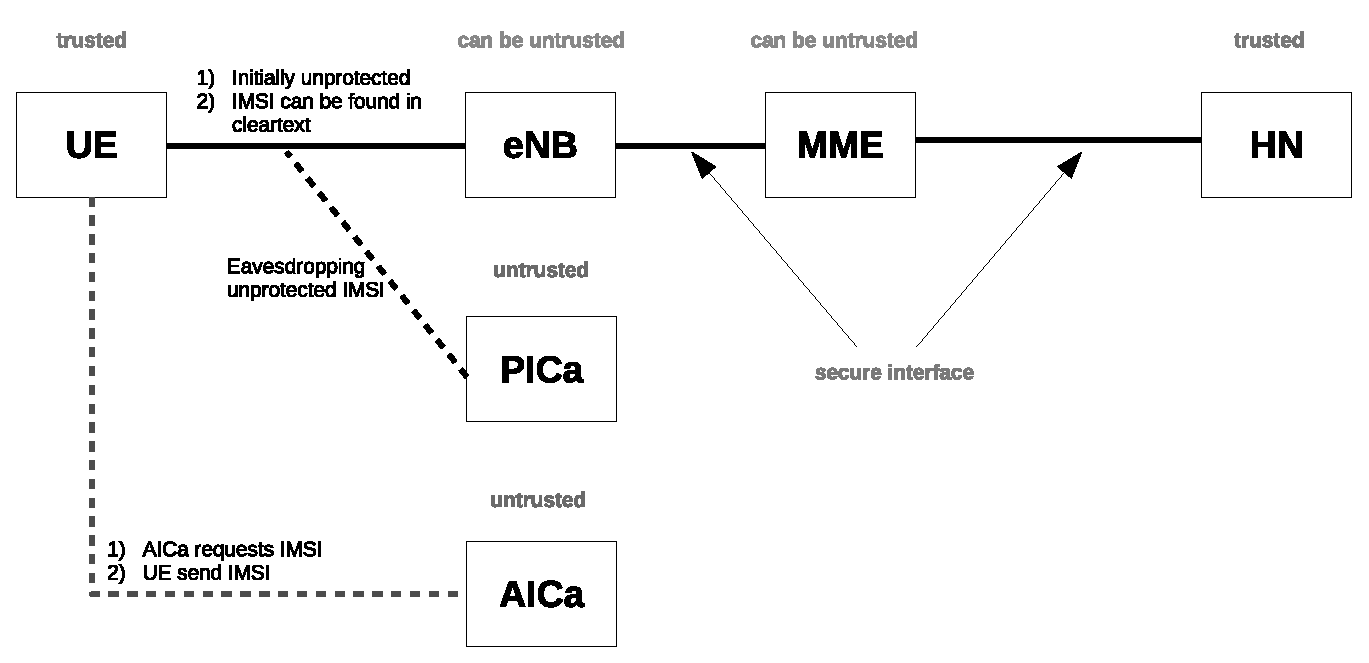
\includegraphics[width=.98\textwidth]{security_architecture_abstraction.eps}
% figure caption is below the figure
%%\caption{High-level security architecture}
%%\label{fig:security_architecture_abstraction}       % Give a unique label
%%\end{center}
%%\end{figure}


\subsubsection{Solutions Against IMSI catchers}
One approach of protecting IMSI privacy is to use a temporary identifier instead of the actual IMSI and keep changing the temporary identifier at a feasible frequency. Note that the temporary identifier has to be assigned over a confidentiality protected channel and different entities of the network may assign different temporary identifiers to the UE. In the LTE network, the temporary identifier assigned by serving network (SN) is called globally unique temporary identity (GUTI) and the home network (HN) does not assign any temporary identifier to the UE. However, during the initial attachment of a UE to the SN, the UE has neither a GUTI nor a security context with the SN that can assign it with a GUTI. Besides, GUTI can be lost by either one or both of the UE and the SN. This would force the UE to reveal its IMSI to the SN to keep itself from permanently locked out of the network. This problem gives an opportunity to an active IMSI catcher (AIC) who impersonates a legitimate SN and forces the UE to run the initial attachment protocol. This also gives an opportunity to a passive IMSI catcher (PIC) to eavesdrop the IMSI sent in clear text. Solutions \cite{pseudonym_valtteri_philip, pseudonym_ericsson} have been proposed by using temporary IMSI known as pseudonym assigned by the HN. 

\section{Categories of Solutions}
We focus on the solutions using cryptographic techniques. So, we look into the different categories of encryption and see their pros and cons. Modern-day encryption can be broadly categorized into two categories depending on how the keys are used to encrypt and decrypt the message. In symmetric-key encryption the sender and receiver share a secret key which is used for both encryption and decryption. In public-key encryption the receiver has a pair of keys. One of the keys is public and the other is private. The public key is used by the sender to encrypt the message and the private key is used by the receiver to decrypt the message. While the challenge in symmetric key encryption is to create a key known only by the sender and receiver but no one else, one major challenge in public-key encryption is to authenticate the public key.
\begin{figure*}
\begin{center}
% Use the relevant command to insert your figure file.
% For example, with the graphicx package use
  \includegraphics[width=.98\textwidth]{ibc_in_jargon_of_crypto.eps}
% figure caption is below the figure
\caption{IBE in the Jargon of Encryption}
\label{fig:ibe_in_the_jargon_of_cryptography}       % Give a unique label
\end{center}
\end{figure*}

Public-key encryption can be further categorized into three more subcategories based on the authentication mechanism used to verify the public keys:
\begin{enumerate}
\item Certificate based encryption
\item Root-key based encryption
\item IBE
\end{enumerate} 
Figure \ref{fig:ibe_in_the_jargon_of_cryptography} shows this categorization with advantages and disadvantages of the respective categories. Please note that this classification is drawn considering only the encryption operation. Different classifications could be drawn based on other cryptographic operations for example digital signature, hashing or MAC. Nonetheless, we use this classification, because encryption is the most relevant cryptographic operation for identity confidentiality. We want to come up with at least one solution using each of the possible subcategories of public-key encryption. We believe all public-key encryption based solution fall into one of these three subcategories with high probability. It makes sense to first compare categories and only in the second phase, compare individual solutions inside each category. We also believe, this is a systematic approach which makes the comparative evaluation easier and meaningful.


In the certificate based encryption, the public key is signed by a trusted third party. The sender has to be pre-provisioned with the root certificate so that the sender can authenticate the public key of the receiver. In the root-key based encryption, no runtime authentication of the public key is required, because a very limited number of public keys are used in the system and all the senders are pre-provisioned with all the existing public keys. In IBE, the public key of a receiver is computed from the identity of the receiver and the public key of a trusted third party. The public key of the trusted third party has to be provisioned to sender. The private key of the receiver is computed from the identity of the receiver and the private key of the trusted third party. The private key of the receiver has to be provisioned to the receiver by the trusted third party.



\section{Conclusion}
This part presents the key findings in substance. Avoid simple enumeration of the following material. It is desirable to provide a link to existing articles and grants. 

\section*{Acknowledgment}
This section is not numbered. You may wish to express gratitude here.

\begin{thebibliography}{6}

\bibitem{NGMN_white_paper} NGMN 5G White Paper V1.0 [cited Jan, 2017]. Available at: https://www.ngmn.org/uploads/media/\\NGMN\_5G\_White\_Paper\_V1\_0.pdf

\bibitem{TR33899} 3GPP TR 33.899 V0.6.0 [cited Jan, 2017]. Available at: https://portal.3gpp.org/desktopmodules/Specifications/\\SpecificationDetails.aspx?specificationId=3045

\bibitem{TS23003} 3GPP TS 23.003 V14.2.0 [cited Jan, 2017]. Available at: https://portal.3gpp.org/desktopmodules/Specifications/\\SpecificationDetails.aspx?specificationId=729

\bibitem{TR21905} 3GPP TR 21.905 [cited Jan, 2017]. Available at: https://portal.3gpp.org/desktopmodules/Specifications/\\SpecificationDetails.aspx?specificationId=558


\bibitem{pseudonym_ericsson} Karl Norrman, Mats N\"aslund, Elena Dubrova: Protecting IMSI and User Privacy in 5G Networks. 2nd International Workshop on 5G Security

\bibitem{pseudonym_valtteri_philip} Philip Ginzboorg,  Valtteri Niemi: Privacy of the long-term identities in cellular networks. Proceedings of the 9th EAI International Conference on Mobile Multimedia Communications
Pages 167-175


\bibitem{Cover}
\textit{(Example for books)} T.M.Cover and J.A. Thomas, \emph{Elements of Information Theory}. New York: Wiley, 1991.

\bibitem{Dobrushin}
\textit{(Example for articles)} R.L. Dobrushin, ``Optimum information transmission through a channel with unknown parameters'',  \emph{Radiotech.Electron.}, vol.4, Dec.1959, pp. 1951-1956.

\bibitem{Blachman}
\textit{(Example for articles)} N.M. Blachman, ``Communication as a game'', \emph{in Proc. WESCON Conf.}, Aug. 1957, pp. 61-66.

\bibitem{IEEE}
\textit{(Example for web-links)} IEEE official website, Manuscript Templates for Conference Proceedings, Web: http://www.ieee.org/conferences\_events/conferences/publishing/templates.\newline html.

\bibitem{Elissa}
\textit{(Example for unpublished references)} K. Elissa, ``Title of paper if known'', unpublished.

\bibitem{Nicole}
\textit{(Example for references have been accepted for publication)} R. Nicole, ``Title of paper with only first word capitalized'', J. Name Stand. Abbrev., in press.

\end{thebibliography}

\end{document}